\documentclass{school}

\subject{NW2 Physik}
\title{Strahlung und Zerfall}
\subtitle{Jahr 4 \-- Semester 2 \-- Test 4}

\author{Markus Reichl}

\begin{document}

\maketitle
\tableofcontents
\newpage

\section{Atommodelle}
\subsection{Bohr'sches Atommodell}
Atome bestehen bei diesem Modell aus einem positiv geladenen Atomkern und negativ geladenen Elektronen, die den Atomkern auf geschlossenen Bahnen umkreisen.\cite{wikipedia-bohr}

\begin{figure}[!ht]
\centering
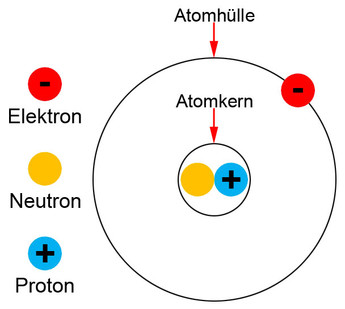
\includegraphics[width=0.25\textwidth]{einfaches-atommodell-a3.jpg}\\
\caption[https://www.sps-lehrgang.de/atommodelle/]{Bohr'sches Atommodell}
\end{figure}

\subsubsection[Bohr'sche Postulate]{Bohr'sche Postulate\protect\footnote{Eine wissenschaftliche Annahme oder Behauptung}}
\begin{enumerate}
    \item Elektronen umkreisen strahlungsfrei den Atomkern
    \item Beim Übergang von Elektronen zwischen zwei Elektronenbahnen wird Energie abgestrahlt oder aufgenommen
\end{enumerate}

\subsubsection{Festkörper}
Bei Festkörpern sind Atome in einem Kristallgitter angeordnet.
Stahl, als Beispiel, hat im Eisengitter ein C-Atom angeordnet.

\begin{figure}[!ht]
    \centering
    \begin{subfigure}[!ht]{0.2\textwidth}
        \centering
        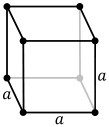
\includegraphics[width=0.6\textwidth]{cubic.png}
        \caption[https://de.wikipedia.org/wiki/Bravais-Gitter]{Primitiv}
    \end{subfigure}
    \begin{subfigure}[!ht]{0.2\textwidth}
        \centering
        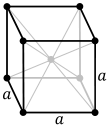
\includegraphics[width=0.6\textwidth]{cubic-centered.png}
        \caption[https://de.wikipedia.org/wiki/Bravais-Gitter]{Raumzentriert}
    \end{subfigure}
    \begin{subfigure}[!ht]{0.2\textwidth}
        \centering
        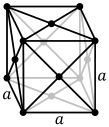
\includegraphics[width=0.6\textwidth]{cubic-face-centered.png}
        \caption[https://de.wikipedia.org/wiki/Bravais-Gitter]{Flächenzentriert}
    \end{subfigure}
    \caption[https://de.wikipedia.org/wiki/Bravais-Gitter]{Kubische Gitter}
\end{figure}

\begin{enumerate}[label= (\alph*)]
    \item \textbf{Kubisch primitives Gitter} Es ist kein weiteres C-Atom enthalten
    \item \textbf{Kubisch raumzentriertes Gitter} Das C-Atom befindet sich im Zentrum
    \item \textbf{Kubisch flächenzentriertes Gitter} Jede Fläche enthälft ein C-Atom in der Mitte
\end{enumerate}
\subsection{Wellenmodell}

\section{Quantenphysik}
Nach Max Planck, ist jede Strahlung aus Quanten zusammengesetzt. Quanten sind Objekte, welche durch einen Zustandswechsel (meist Energie) erzeugt werden.

\subsection{Plancksches Wirkungsquantum}
Das Planksche Wirkungsquantum $h$, beschreibt das Verhältnis von Energie $E$ und Frequenz $f$ eines Photons\footnote{In diesem Kontext auch als Lichtquant bekannt}.
$$E = h * f$$
$$f = \frac{c}{\lambda}$$
\begin{center}
    \begin{tabular}{l l l}
        $h$ &\dots Wirkungsquantum & $6.63 * 10^{-34} Js$\\
        $f$ &\dots Frequenz & ${s}$\\
        $f$ &\dots Wellenlänge & ${m}$
    \end{tabular}
\end{center}

\subsubsection{Bsp.: Masse eines Photons}
Einsteins Äquivalenzenprinzip und das Plancksche Wirkungsquantum können gleichgesetzt werden, womit sich die Masse eines Photons, bei einer bestimmten Wellenlänge (hier $500nm$) errechnen lässt.
$$E = m * c^2$$
\begin{center}
    \begin{tabular}{l l l}
        $E$ &\dots Energie & $J$\\
        $m$ &\dots Masse & $kg$\\
        $c$ &\dots Lichtgeschwindigkeit & $3*10^8 {m}{s^2}$
    \end{tabular}
\end{center}
\vspace{0.8 em}
$$h * f = m * c^2$$
$$m = \frac{6.63 * 10^{-34} * 500 * 10^{-9}}{c^2}$$
$$m \approx 44.2 * 10^{-34}g $$

\newpage
\subsection{Bsp.: Fotozelle}
Eine Fotozelle spricht an, wenn sie mit Licht der Leistung $P = 10^{-18}$ Watt bestrahlt wird.
Wie viele Lichtquanten $N$ (Photonen) der Wellenlänge $\lambda = 6.44 * 10^{-7}$ Meter fallen pro Sekunde auf die Fotozelle?
$$E = P * t$$
Die Energie gilt der Anzahl der Photonen $N$, diese wird einfach als Faktor des Wirkungsquantum hinzugefügt.
$$E = N * h* f$$
$$f = \frac{c}{\lambda}$$
$$P * t = N * \frac{h * c}{\lambda}$$
$$N = \frac{P * t * \lambda}{h * c}$$
$$N = \frac{10^{-18} * 1 * 6.44 * 10^{-7}}{6.63 * 10^{-34} * 3 * 10^8}$$
\vspace{0.8 em}
$$N \approx 3.238 \text{ Lichtquanten}$$

\subsubsection{Bsp.: Glühbirne}
5 Prozent der elektrischen Leistung einer 60 Watt Glühbirne, wird in Licht der Wellenlänge $\lambda = 5.6 * 10^{-7}$ Meter umgewandelt.
Wie viele Lichtquanten dieser Wellenlänge werden pro Sekunde ausgesandt?
$$N = \frac{P* t * \lambda}{h * c}$$
$$N = \frac{60 * 1 * 5.6 * 10^{-7}}{6.63 * 10^{-34} * 3 * 10^8}$$
\vspace{0.8 em}
$$N \approx 0.43*10^{18} \text{ Lichtquanten}$$

\newpage
\subsection{Unschärferelation}
Jede Steigerung der Genauigkeit in der Ortsbestimmung reduziert die Genauigkeit in der Geschwindigkeitsbestimmung.
\vspace{0.8 em}\\
Diese Ungenauigkeit ist prinzipieller Natur und kann durch verbesserte Technologien nicht reduziert werden.\\
Die Unschärferelation gilt auch für makroskopische Körper.
\paragraph{Heisenberg}
$$\Delta x * \Delta p \ge \frac{h}{2\pi}$$
\vspace{0.25 em}
$$p = m * v$$

\begin{center}
    \begin{tabular}{l l l}
        $h$ &\dots Plancksches Wirkungsquantum & $6.63 * 10^{-34} Js$\\
        $p$ &\dots Impuls & ${kg * m}{s}$\\
        $m$ &\dots Masse & ${kg}$\\
        $v$ &\dots Geschwindigkeit & ${m}{s}$\\
        $\Delta x$ &\dots Unschärfe des Ortes & ${m}$\\
        $\Delta p$ &\dots Unschärfe des Impulses & ${kg * m}{s}$
    \end{tabular}
\end{center}

\subsubsection{Bsp.: Auto}
Ein Auto mit der Masse $m = 1200 kg$ bewegt sich mit $v = 170 \frac{km}{h}$.
Welche Ungenauigkeit tritt bei der Bestimmung des Ortes mindestens auf?
$$\Delta x * \Delta p \ge \frac{h}{2\pi}$$
Der Impuls kann in diesem Fall genau über $m * v$ bestimmt werden, da es sich um die minimale Ungenauigkeit handelt wird das $\ge$ zu einem $=$.
$$\Delta x = \frac{h}{2\pi * m * v}$$
$$\Delta x = \frac{6.63 * 10^{-34}}{2\pi * 1200 * \frac{170}{3.6}}$$
$$\Delta x \approx 1.76 * 10^{-39} m$$

\newpage
\section{Röntgenröhre}
\begin{figure}[!ht]
\centering
    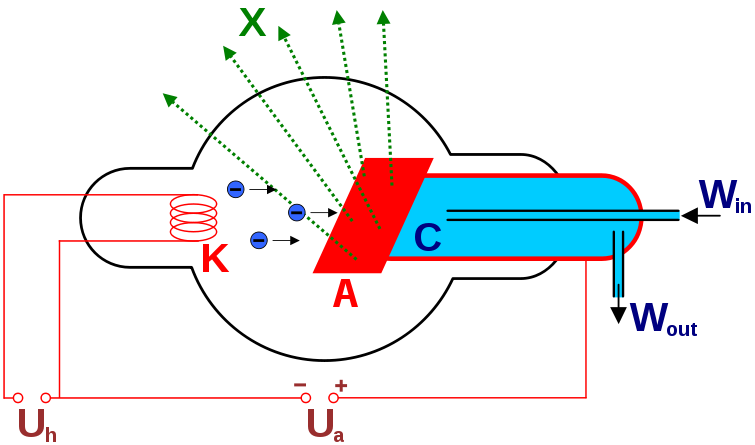
\includegraphics[width=0.45\textwidth]{roentgen-roehre.png}
    \caption[https://de.wikipedia.org/wiki/Röntgenröhre]{Röntgen Röhre}
\end{figure}
\begin{center}
    \begin{tabular}{l l l}
        $U$ &\dots Spannung & $V$\\
        $X$ &\dots Röntgenstrahlung &\\
        $K$ &\dots Kathode &\\
        $A$ &\dots Anode &
    \end{tabular}
\end{center}
Die Anode besteht aus einem Material mit hohem Atomgewicht (Wolfram oder Kupfer) und verursacht charakteristische Eigenstrahlung. Durch die Hochspannung innerhalb der Röhre wird zudem Bremsstrahlung verursacht, welche Elektronen verlangsamt.

\subsection{Energie des Elektrons}
Die Energie eines Elektrons kann durch folgende Formel ausgedrückt werden.
$$E = e * U$$
\begin{center}
    \begin{tabular}{l l l}
        $E$ &\dots Spannung & $J$\\
        $e$ &\dots Elementarladung & As\footnote{Amperesekunden}\\
        $U$ &\dots Spannung & $V$
    \end{tabular}
\end{center}

\newpage
\subsubsection{Bsp.: Geschwindigkeit von $e^-$}
Welche Geschwindigkeit haben $e^-$ in einer Röntgenröhre, wenn deren Strahlen eine Wellenlänge $\lambda$ von $10^{-10}m$ aufweisen und welche Spannung ist dafür notwendig?
\paragraph{(a)}
Zur Berechnung der Geschwindigkeit $v$ muss diese zuerst über eine andere Formel eingebaut werden. Dieses Beispiel nutzt hierzu $E = \frac{m*v^2}{2}$ und $E = h * f$ mit $f = \frac{c}{\lambda}$.
$$\frac{m*v^2}{2} = \frac{h * c}{\lambda}$$
~\\
Nun kann einfach auf die Geschwindigkeit umgeformt und eingesetzt werden.
$$v = \sqrt{\frac{2 * h * c}{m * \lambda}}$$
$$v = \sqrt{\frac{2 * 6.63*10^{-34}*3*10^8}{9.11 * 10^{-31} * 10^{-10}}} \approx 6.6 * 10^7 \frac{m}{s}$$
\paragraph{(b)}
Die notwendige Spannung ergibt sich aus der Formel $E = e * U$, wobei erneut mit der Formel $E = h * f$ mit $f = \frac{c}{\lambda}$ gleichgesetzt werden kann.
$$e * U = \frac{h * c}{\lambda}$$
$$U = \frac{h * c}{e * \lambda}$$
$$U = \frac{6.63 * 10^{-34} * 3 * 10^8}{9.11 * 10^{-31} * 10^{-10}} \approx 12.4 kV$$

\newpage
\section{Radioaktivität}
\begin{quote}
``Radioaktivität ist die Eigenschaft instabiler Atomkerne, spontan ionisierende Strahlung auszusenden.'' \cite{wikipedia-radio}
\end{quote}
Radioaktive Elemente haben die Fähigkeit ihre Kerne unter Aussendung von Strahlung umzuwandeln. Dieser Prozess unterscheidet mehrere Fälle.

\paragraph{Alpha Zerfall}
Aus einem Atom wird ein Alpha Teilchen\footnote{Ein Helium Atom mit 2 Protonen und 2 Neutronen} $H^4_2$ herausgelöst.
\subparagraph{Bsp.:} $U^{235}_{92} \to Th^{231}_{90} + H^4_2$

\paragraph{Beta Zerfall}
Aus einem Atom wird ein Beta Teilchen\footnote{Elektron mit $r=10^8 \frac{m}{s}$} $e^-$ herausgelöst.
\subparagraph{Bsp.:} $U^{235}_{92} \to U^{235}_{92} + e^-$

\paragraph{Gamma Strahlung}
Anstatt von Teilchen wird hier elektromagnetische Strahlung in Form von Photonen ausgesandt.

\subsection{Auswirkungen}
\begin{tabular}{l|l|l|l|l}
    Art & Strahlung & Reichweite & Schaden & Schutz\\
    \hline
    $\alpha$-Strahlung & $\alpha$-Teilchen & Gering & Hoch & Papier\\
    $\beta$-Strahlung & $\beta$-Teilchen & Mittel & Mittel & Metallplatte \\
    $\gamma$-Strahlung & Elektromagnetische Strahlung & Hoch & Gering & Bleiwand
\end{tabular}

\subsection{Wechselwirkung von Strahlung und Materie}
\begin{figure}[!ht]
\centering
    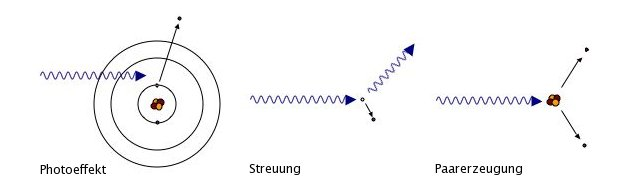
\includegraphics[width=0.8\textwidth]{strahlung-materie.jpg}
    \caption[http://www.sebastian-hess.eu]{Strahlung und Materie}
\end{figure}

\section{Zerfallsgesetze}
Betrachtet man ein radioaktives Präparat mit anfänglich $N_{0}$ Atomkernen und der Aktivität $A$, so gilt folgendes für die Anzahl $N$ der in der Zeit $t$ noch nicht zerfallenen Kerne.
$$A = -\frac{dN}{dt} \text{ mit } A = \lambda * N$$
Durch Integration erhält man damit folgende formel.
$$N(t) = N_0 * e^{-\lambda * t}$$
\subsection{Mittlere Lebensdauer}
Die Zerfallskonstante $\lambda$ ist der Kehrwert der mittleren Lebensdauer $\tau = \frac{1}{\lambda}$, also der Zeit, nach der die Zahl der Atome sich um den Faktor $e$ verringert hat. $\tau$ unterscheidet sich von der Halbwertszeit $T_{1/2}$ nur um den konstanten Faktor $ln(2)$.
$$N(t) = N_0 * e^{\frac{-ln(2)}{T_{1/2}} * t}$$
\begin{center}
    \begin{tabular}{l l l}
        $T_{1/2}$ &\dots Halbwertszeit & \small{(Zerfallsakte)}\\
        $N$ &\dots Atomkerne &\\
        $A$ &\dots Aktivität &\\
        $t$ &\dots Zeit & $s$
    \end{tabular}
\end{center}

\newpage
\subsubsection{Bsp.: Holz}
Das Holz lebender Bäume enthält unabhängig von der Art des Baumes so viel $^{14}_{16}C$, dass sich im Mittel $15.3$ Zerfallsakte je Minute und je Gramm Kohlenstoffgehalt ereignen. In einer Höhle wurde Holzkohle gefunden, die nur noch $12.5$ Zerfallsakte je Minute und je Gramm Kohlenstoffgehalt aufwies.
\begin{enumerate}[label= (\alph*)]
    \item Wie alt muss die Holzkohle sein, wenn die Halbwertszeit $T_{14} = 5568$ Jahre angesetzt wird.
    \item Welche Unsicherheit ergibt sich für das errechnete Alter, wenn die Halbwertszeit auf $30$ Jahre ungenau ist, also $T_14 = 5568 \pm 40$ Jahre betragen kann.
\end{enumerate}
\paragraph*{(a)}
Im Text werden die jeweiligen Zerfallsakte, sowie die Halbwertszeit angegeben.
$$T_{14} = 5568 \text{ Jahre}$$
$$N_0 = 15.3 \frac{T_{1/2}}{m * t}$$
$$N(t) = 11.5 \frac{T_{1/2}}{m * t}$$
~\\
Diese Werte können einfach in die Zerfallsformel eingesetzt werden. Das Alter des Holzes aus der Höhle kann dann durch umformen auf $t$ errechnet werden.
$$N(t) = N_0 * e^{\frac{-ln(2)}{T_1/2} * t}$$
$$11.5 = 15.3 * e^{\frac{-ln(2)}{5568} * t}$$
$$ln(\frac{11.5}{15.3}) = \frac{-ln(2)}{5568} * t$$
$$- 5568 * \frac{ln(\frac{11.5}{15.3})}{ln(2)} = t$$
$$- 5568 * 2293.45 = t$$
$$t = 1624 \text{ Jahre}$$
\paragraph*{(b)}
Bei der Ungenauigkeit handelt es sich um eine Variation der Halbwertszeit, welche einfach zum ursprünglichen Wert addiert, bzw. zubtrahiert wird.
$$T_{14} = 5568 \pm 30 \text{ Jahre}$$
$$- (5568 \pm 30) *2293.45 = t$$
$$t_{-30} = 1616 \text{ Jahre}$$
$$t_{+30} = 1933 \text{ Jahre}$$

\newpage
\begin{thebibliography}{9}
    \bibitem{wikipedia-bohr} https://de.wikipedia.org/wiki/Bohrsches\_Atommodell
    \bibitem{wikipedia-radio} https://de.wikipedia.org/wiki/Radioaktivität
    \bibitem{wikipedia-zerfall} https://de.wikipedia.org/wiki/Zerfallsgesetz
\end{thebibliography}

\listoffigures

\end{document}
